\documentclass{article}
\usepackage{longtable} % 支持长表格
\usepackage{verbatim}  % 支持代码
\usepackage{geometry}  % 控制页面布局
\geometry{a4paper, margin=1in}
\usepackage{amsmath}
\usepackage{graphicx}
\usepackage{listings}
\usepackage{pythonhighlight}
\usepackage[UTF8]{ctex}


\title{第三次作业}
\author{时伟杰}
\date{\today}
\begin{document}

\maketitle

\section{Python简介}
Python是一种通用的高级编程语言,由吉多·范罗苏姆于1991年首次发布。它以简洁、易读的语法和强大的功能而著称,这使得它在各种编程领域都极具吸引力。Python的设计理念强调代码的可读性和简洁性,尽可能减少了程序员的工作量。Python具有动态类型、自动内存管理和支持多种编程范式,包括面向对象、过程式和函数式编程。

Python的标准库丰富,涵盖了从文件操作、网络编程到数据处理等各种功能,减少了重复造轮子的需要。在数据科学和机器学习领域,Python几乎是首选语言。它拥有强大的第三方库和工具,如NumPy、Pandas、Matplotlib和Scikit-Learn,这些库提供了数据处理、分析和可视化的能力。此外,Python在Web开发方面也表现出色,框架如Django和Flask帮助开发者快速构建高效、可靠的Web应用。

Python的应用领域非常广泛,包括Web开发、数据科学、自动化脚本、游戏开发、人工智能等。由于其开源特性,Python有一个活跃的社区,这为用户提供了大量的资源和支持。Python的包管理工具pip使得安装和管理第三方库变得简单方便。

\newpage
\section{实例演示}

\begin{longtable}{|c|p{10cm}|l|}
\hline
编号 & Python 操作 & 说明 \\
\hline
1 & \verb|print("hello world")| & 打印 \\
\hline
2 & \verb|print("He said \"Let's go!\"")| & 反斜杠打印特殊字符 \\
\hline
3 & \verb|print("""天生我材必有用| \newline \verb|千金散尽还复来""")| & 三引号打印 \\
\hline
4 & \verb|print("hello world".title())| & 首字母大写 \\
\hline
5 & \verb|username = "wj"| & 变量名赋值 \\
\hline
6 & \verb|message = f"{username} welcome to Python Programming"| & f字符串输出 \\
\hline
7 & \verb|import math| \newline \verb|print(math.log2(8))| & 调用 math 函数库 \\
\hline
8 & \verb|# 这是一段注释| & 注释 \\
\hline
9 & \verb|shopping_list = ["手机","键盘"]| & 列表 \\
\hline
10 & \verb|shopping_list.append("显示器")| & 列表添加元素 \\
\hline
11 & \verb|shopping_list.remove("显示器")| & 列表移除元素 \\
\hline
12 & \verb|print(len(shopping_list))| & 打印列表长度 \\
\hline
13 & \verb|print(shopping_list[0])| & 打印列表第一个元素 \\
\hline
14 & \verb|num_list = [6,2,3,4,5]| & 数字列表 \\
\hline
15 & \verb|print(max(num_list))| & 打印最大值 \\
\hline
16 & \verb|min(num_list)| & 打印最小值 \\
\hline
17 & \verb|sorted(num_list)| & 排序 \\
\hline
18 & \verb|for num in num_list:| \newline \verb|if num > 3:| \newline \verb|print("yes")| & for 循环的使用 \\
\hline
19 & \verb|for i in range(len(num_list)):| \newline \verb|num_list[i] = num_list[i] + 1| \newline \verb|print(num_list)| & 所有列表元素加 1 \\
\hline
20 & \verb|if shopping_list[0] == "手机":| \newline \verb|print("我要先买手机")| \newline \verb|elif shopping_list[1] == "电脑":| \newline \verb|print("我第二个买电脑")| \newline \verb|else:| \newline \verb|print("我不买电脑")| & if 条件语句使用 \\
\hline
21 & \verb|contacts = {"小明":"1370000","小花":"1370001"}| \newline \verb|print(contacts["小明"])| & 字典的使用 \\
\hline
22 & \verb|pil_im = Image.open('image.jpg')| & 读取图像并生成图像对象 \\
\hline
23 & \verb|gray_im = pil_im.convert('L')| & 将彩色图像转换为灰度图 \\
\hline
24 & \verb|pil_im.save('new_image.png')| & 保存图像,并可选择不同的格式 \\
\hline
25 & \verb|pil_im.thumbnail((128,128))| & 创建图像缩略图 \\
\hline
26 & \verb|cropped_im = pil_im.crop((100,100,400,400))| & 裁剪图像的指定区域 \\
\hline
27 & \verb|pil_im.paste(cropped_im, (50, 50))| & 一幅图像粘贴到另一幅图像上 \\
\hline
28 & \verb|rotated_im = pil_im.rotate(45)| & 旋转图像 \\
\hline
29 & \verb|plt.imshow(pil_im)| & 绘制图像 \\
\hline
30 & \verb|plt.hist(pil_im.convert('L').ravel(), bins=256)| & 生成图像灰度直方图 \\
\hline
31 & \verb|gray_array = np.array(pil_im.convert('L'))| & 灰度转换为数组 \\
\hline
32 & \verb|resized_im = pil_im.resize((200, 200))| & 调整图像大小 \\
\hline
33 & \verb|flipped_im = np.flipud(np.array(pil_im))| & 实现图像翻转 \\
\hline
34 & \verb|blurred_im = gaussian_filter(np.array(pil_im), sigma=2)| & 高斯模糊 \\
\hline
35 & \verb|edges = ndimage.sobel(np.array(pil_im.convert('L')))| & 计算图像边缘 \\
\hline
36 & \verb|labeled, num_objects = ndimage.label(binary_image)| & 对象计数 \\
\hline
37 & \verb|V, S, mean_im = pca(immatrix)| & 主成分分析 \\
\hline
38 & \verb|denoised_im = denoise_image(pil_im)| & 自定义图像去噪算法 \\
\hline
39 & \verb|equalized_im = exposure.equalize_hist(np.array(pil_im))| & 直方图均衡化 \\
\hline
40 & \verb|mean_im = np.mean(image_list, axis=0)| & 多幅图像进行像素均值计算 \\
\hline
\end{longtable}
\section{截图示例}

\begin{figure}[htbp]
\centering
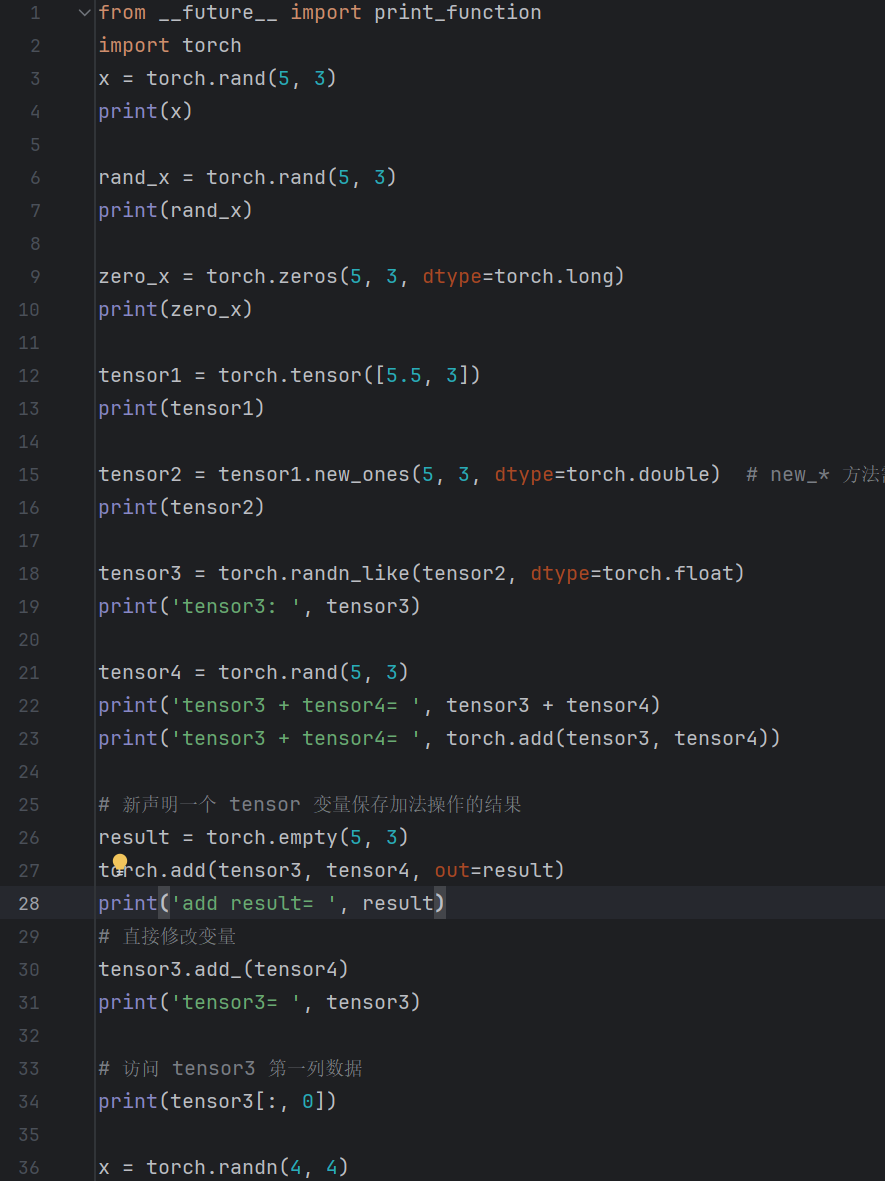
\includegraphics[width=0.7\textwidth]{1.png}
\caption{截图1:某Python代码运行结果}
\label{screenshot1}
\end{figure}

\begin{figure}[htbp]
\centering
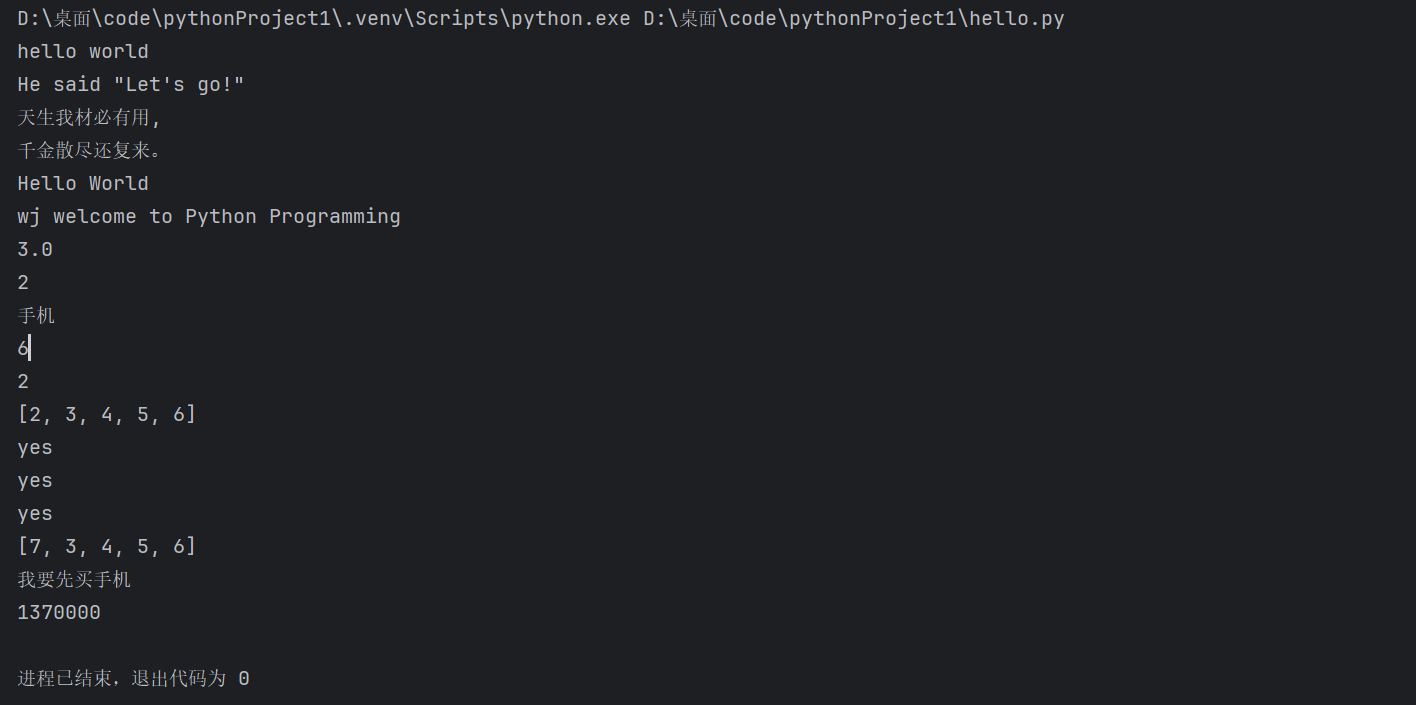
\includegraphics[width=0.8\textwidth]{2.png}
\caption{截图2:某图像处理效果}
\label{screenshot2}
\end{figure}

\newpage
\section{心得体会}
学习Python编程以及Python在计算机视觉领域的应用,让我逐渐体会到了它的简洁和高效。在最开始学习时,Python的简单语法让我感到惊喜。相比于C++等更底层的编程语言,Python的代码几乎没有繁琐的语法结构,这让编程变得不再那么复杂,特别是在处理图像时,少量的代码就能实现复杂的操作。

例如,使用PIL库读取和显示一幅图像,只需几行代码即可完成。随着学习的深入,我发现Python在计算机视觉领域拥有极为丰富的库支持。像OpenCV这种功能强大的视觉库,不仅提供了传统的图像处理算法,还支持视频处理、对象检测等高级功能。通过学习这些库,我能快速实现一些经典的视觉算法,比如边缘检测、图像滤波等。

Python语言的模块化设计让我感受到其强大的扩展性。在图像处理过程中,我时常需要将视觉处理与其他功能结合,比如读取文件、存储结果,甚至是将图像与深度学习模型结合。而Python通过导入特定的模块,可以在几乎不增加代码复杂度的情况下完成这些任务。比如,使用NumPy库,我可以轻松实现大规模图像数据的矩阵运算,而不需要手动编写复杂的矩阵操作代码,这种模块化的特性大大提高了开发效率。

在夏季学期的时候,我同时上了一门国际课程——计算机视觉导论。在学习过程中,我逐渐意识到,计算机视觉不仅仅是图像的处理,更是通过视觉来理解世界。Python的开放性使得它与深度学习框架(如TensorFlow、PyTorch)完美结合,这让我能够利用AI技术解决更复杂的视觉问题,比如图像分类、物体检测等。通过调用预训练模型,我甚至可以在几分钟内构建一个功能齐全的图像识别应用,这种视觉与AI的结合为未来提供了无限的可能性。

Python让我体会到了编程的简洁与高效,尤其是在视觉处理这个复杂的领域,通过Python,我能够以一种更加轻松、愉快的方式来探索计算机视觉的魅力。

\end{document}